
\documentclass{llncs} %
\setcounter{tocdepth}{4}
\usepackage{geometry}
\geometry{
  letterpaper,         % or letterpaper
  textwidth=6.5in,  % llncs has 12.2cm
  textheight=9in, % llncs has 19.3cm
  heightrounded,   % integer number of lines
  hratio=1:1,      % horizontally centered
  vratio=2:3,      % not vertically centered
}
\linespread{1.6}

\author{Martin D. Muggli}
\title{A Survey of Genome Sequence Assembly Methods}
\institute{Computer Science Department, Colorado State University}

\begin{document}
\maketitle

%\begin{abstract}
Modern genome sequencing is largely based on a process of randomly breaking replicated copies of a genome into fragments, using various technologies to capture the nucleotide sequence within these fragments (resulting in strings known as reads), and then using assembly software to attempt to reconstruct the original genome sequence from the reads.
This process is challenging as genomes contain repeated regions, and repeated regions much longer than read length confound assemblers, limiting their ability to completely and correctly reconstruct genomes successfully.
Correct and complete genome assembly is important because genomes encode elements that cooperate with others in close proximity, and thus not just the content, but  genome structure has important biological implications.
To the extent quality automated genome reconstruction is possible, there is an additional challenge of accessibility, as some of the most successful assembly software requires unusually high-end servers or clusters.
This limits their usefulness to biologists with access and skill to use such machines and hence more efficient computational techniques are of value.
Beyond efficiency and correctness of algorithms, there is interplay between computational approach, sequencing technology (which vary in read length, accuracy, applicability, and level of detail), and the assembly quality that may result.
In this report, we will expand on the concepts introduced here and review a selection of modern computational assembly tools, the sequence data on which they operate, and discuss important advantages, limitations, and possible extensions of them as well as their relationship to each other in the context of the sequence assembly problem.
%\end{abstract}

%\tableofcontents

\section*{Preliminaries} \label{prel:vari}

As previously mentioned, in 2017 Muggli et al.~\cite{vari} presented $\vari$, which is a representation of the colored de Bruijn graph using BWT.  Our proposed method, $\ours$, efficiently merges de Bruijn graphs that are represented in this manner. Therefore, we first define some basic notation and definitions concerning BWT, then we show how the de Bruijn graph can be stored using BWT, and finally, we show how the {\em colored} de Bruijn graph can be stored succinctly.  We refer the reader to the full paper by Muggli et al.~\cite{vari} for a more detailed discussion of the representation.   

\subsection*{Basic Definitions and Terminology} %\subsection{sec:basic}

Here, we begin with some basic definitions related to our representation.  Throughout we consider a string $\X = \X[1..n] = \X[1]\X[2]\ldots
\X[n]$ of $|\X| = n$ symbols drawn from the alphabet $[0..\sigma-1]$.
%We assume $\X[n]$ is a special ``end of string'' symbol, \$, smaller than
%all other symbols in the alphabet.
For $i=1,\ldots,n$ we
write $\X[i..n]$ to denote the {\em suffix} of $\X$ of length $n-i+1$,
that is $\X[i..n] = \X[i]\X[i+1]\ldots \X[n]$.  
%We will often refer to suffix $\X[i..n]$ simply as ``suffix $i$''. 
Similarly, we write
$\X[1..i]$ to denote the {\em prefix} of $\X$ of length $i$.
$\X[i..j]$ is the {\em substring} $\X[i]\X[i+1]\ldots \X[j]$ of $\X$
that starts at position $i$ and ends at $j$. 
%By $\X[i..j)$ we
%denote $\X[i..j-1]$.  If $j < i$ we
%define $\X[i..j]$ to be the empty string, also denoted by
%$\varepsilon$.

\paragraph*{Suffix arrays and suffix array intervals.}
The suffix array~\cite{mm1993} $\SA_{\X}$ (we drop subscripts when
they are clear
from the context) of a string $\X$
is an array $\SA[1..n]$ which
contains a permutation of the integers $[1..n]$ such that $\X[\SA[1]..n]
\prec \X[\SA[2]..n] \prec \cdots \prec \X[\SA[n]..n]$.  In other words, $\SA[j] =
i$ if and only if $\X[i..n]$ is the $j^{\mbox{{\scriptsize th}}}$ suffix of $\X$
in lexicographical order. Here, $\prec$ denotes lexicographic precedence.

%The inverse
%suffix array $\ISA$ is the inverse permutation of $\SA$, that is
%$\ISA[i] = j$ iff $\SA[j] = i$.
%Conceptually, $\ISA[i]$ tells us the position of suffix $i$ in $\SA$. 

%Our data structure for colored de Bruijn graphs is based on a succinct representation of individual de Bruijn graphs that was introduced by Bowe et al.~\cite{BOSS12} and which we refer to as the BOSS representation from the authors' initials.  The BOSS representation was in turn based on an adaptation of Ferragina and Manzini's~\cite{FM05} FM-indexes.  Before getting to our description of the succinct colored de Bruijn graph data structure, 
%In the rest of this section 
%we first describe FM-indexes and then explain the BOSS representation.Our explanation of BOSS is particularly simple and may be of independent interest to those wanting to better understand that data structure.
% This new take on BOSS was key to our development of our succinct colored de Bruijn graph. 
% Travis: No it wasn't, it came afterward. :o)

For a string $\Y$, the $\Y$-interval in the suffix array $\SA_{\X}$ is
the interval $\SA[s..e]$ that contains all suffixes having $\Y$ as a
prefix. The $\Y$-interval is a representation of the occurrences of
$\Y$ in $\X$. For a character $c$ and a string $\Y$, the computation
of $c\Y$-interval from $\Y$-interval is called a \emph{left extension}.
%and the computation of $\Y$-interval from ${\Y}c$-interval is called a
%\emph{right contraction}. \emph{Left contraction} and \emph{right
%  extension} are defined symmetrically.

\paragraph*{BWT.} Next, for a string $\Y$, let $\F$ be the list of $\Y$'s characters sorted lexicographically by the suffixes starting at those characters, and $\L$ be the list of $\Y$'s characters sorted lexicographically by the suffixes starting immediately after those characters.  (The names $\F$ and $\L$ are standard for these lists.)  If \(\Y [i]\) is in position $p$ in $\F$ then \(\Y [i - 1]\) is in position $p$ in $\L$.  Moreover, if \(\Y [i] = \Y [j]\) then \(\Y [i]\) and \(\Y [j]\) have the same relative order in both lists; otherwise, their relative order in $\F$ is the same as their lexicographic order.  This means that if \(\Y [i]\) is in position $p$ in $\L$ then (assuming arrays are indexed from 0) in $\F$ it is in position
\[|\{h\,:\,\Y [h] \prec \Y[i]\}| + |\{h\,:\, \L [h] = \Y [i],\ h \leq p\}| - 1\,.\] Finally, notice that the last character in $\Y$ always appears first in $\L$.  It follows that we can recover $\Y$ from $\L$, which is the famous {\em Burrows-Wheeler Transform (BWT)}~\cite{bw1994} of $\Y$.


\paragraph*{FM-index and backward seach.}  Ferragina and Manzini~\cite{fm2005} first  realized BWT can be used for indexing in addition to compression.   Hence, if we know the range \(\BWT (\Y) [i..j]\) occupied by characters immediately preceding occurrences of a pattern $P$ in $\Y$, then we can compute the range \(\BWT (\Y) [i'..j']\) occupied by characters immediately preceding occurrences of \(c P\) in $\Y$, for any character $c$, since
\begin{eqnarray*}
i' & = & |\{h\,:\,\Y [h] \prec c\}| + |\{h\,:\,\Y [h] = c, h < i\}| \\
j' & =  & |\{h\,:\,\Y [h] \prec c\}| + |\{h\,:\, \Y [h] = c, h \leq j\}| - 1\,.
\end{eqnarray*}
Notice \(j' - i' + 1\) is the number of occurrences of \(c P\) in $S$.  The essential components of an FM-index for $\Y$ are: (1) an array storing \(|\{h\,:\,\Y [h] \prec c\}|\) for each character $c$ and, (2) a {\em rank} data structure for \(\BWT (\Y)\) that quickly tells us how often any given character occurs up to any given position. To be able to locate the occurrences of patterns in $\Y$ (in addition to just counting them), we can use a sampled suffix array of $\Y$ and a bitvector indicating the positions in \(\BWT (\Y)\) of the characters preceding the sampled suffixes.  

Hence, we define the function
$\rank(\Y, c,i)$, for string $\Y$, symbol $c$, and integer $i$, as 
the number of occurrences of $c$ in $\Y[1..i]$. Rank is used in {\em backward search}~\cite{fm2005} in order to compute left extension of a given string, i.e., the previous character. 

 %  It is well known that $\LF[i] = \C[\BWT[i]] + \rank(\BWT,\BWT[i],i)$.  Furthermore, we can compute the left extension using $\C$ and $\rank$.  If $\SA[s..e]$ is the $\Y$-interval,
%containing all the suffixes prefixed with string $\Y$,  then $\SA[\C[c]+\rank(\BWT,c,s),\C[c]+\rank(\BWT,c,e)]$ is the $c\Y$-interval. This is called \emph{backward search}~\cite{fm2005}, and a data structure supporting it is called an {\em FM-index}.


\subsection*{Storage of de Bruijn Graph using BWT} 

Given a de Bruijn graph $G =(V, E)$, we refer to the label of an edge $e \in E$ as the $k$-mer corresponding to it, and denote it as $\elabel(e)$.  Further, given $V$, we define the co-lexicographic (colex) ordering of $V$ as the lexicographic order of their reversed labels ($(k - 1)$-mers).  

We let $\F$ be the edges in $E$ in colex order by their ending nodes, where ties are broken by their starting nodes, and let $\L$ be the edges in $E$ sorted colex by their starting nodes, with ties broken by their ending nodes.  We refer to the ordering of $\L$ as {\em Vari-sorted}. If we are given two edges $e$ and $e'$ that have the same label then we are guaranteed that they have the same relative order in both $\F$ and $\L$; otherwise, their relative order in $\F$ is the same as their labels' lexicographic order.  This means that if $e$ is in position $p$ in $\L$, then in $\F$ it is in position
\[|\{d\,:\,d \in E,\ \elabel (d) \prec \elabel (e)\}| + \]
	\[ |\{h\,:\,\elabel (\L [h]) = \elabel (e),\ h \leq p\}| - 1\,\]
where $\prec$ denotes lexicographic precedence.  We define the edge-$\BWT$ ($\EBWT$) of $G$ to be the sequence of edge labels sorted according to the ordering of the edges in $\L$, so \(\elabel (\L [h]) = \EBWT (G) [h]\) for all $h$. Therefore, if we have an array $D$ storing \(|\{d\,:\,d \in E,\ \elabel (d) \prec c\}|\) for each character $c$ and  a fast rank data structure on \(\EBWT (G)\) then given an edge's position in $\L$, we can quickly compute its position in $\F$.

We let $\B_F$ be the bit vector with a 1 marking the position in $\F$ of the last incoming edge of each node, and let $\B_L$ be the bit vector with a 1 marking the position in $\L$ of the last outgoing edge of each node.  Given a character $c$ and the colex rank of a node $v$, we can use $\B_L$ to find the interval in $\L$ containing $v$'s outgoing edges.  We can then search \(\EBWT (G)\) to find the position of each outgoing edge\footnote{In practice, we incorporate the bits of $B_F$ as flags on \(\EBWT (G)\) and use them to obtain the colex order of $v$ but omit the discussion here for simplicity.  We refer the reader to Bowe et al.~\cite{BOSS} for a full discussion of this aspect and the supplement for our handling here.}. Similarly, we can make similar queries about the incoming edges of a node $v$ in an efficient manner using $\B_F$.  

%In addition, if $B_G$ is  the bit vector with a 0 marking the position in $\F$ of the first incoming edge of each node, we define $\flags$ to be the vector that stores the permutation from $\F$ to $\L$ applied to $\B_G$.  Next, we see how we use $\flags$.  If we are given a character $c$ and the colex rank of a node $v$, we can use $\B_L$ to find the interval in $\L$ containing $v$'s outgoing edges, then we can search in \(\EBWT (G)\) to find the position of the one $e$ labeled $c$.  We need $\flags$ in order to obtain the colex rank of $v$.  Thus, we can find $e$'s position in $\F$, as described above.  Finally, we can use $\B_F$ to find the co-lexicographic rank of $e$'s ending node.  

Therefore, briefly we explained how we can construct and represent a de Bruijn graph $G = (V, E)$ with $\EBWT$, $\B_L$,  and $\B_F$ in a manner that allows for efficient navigation of the graph. An example of this representation is shown in Figure \ref{fig:purple}. Given this representation we can traverse the graph and recover incoming and outgoing edges.   Next, we demonstrate how the labels ($k$-mers) can be recovered using this data structure.

%With the appropriate implementations of the data structures, we obtain the following result:
%\begin{theorem}[Bowe, Onodera, Sadakane and Shibuya, 2012]
%We can store $G$ in \((1 + o (1)) |E| (\lg \sigma + 2)\) bits such that, given a character $c$ and the co-%lexicographic rank of a node $v$, in $O{\log \log \sigma}$ time we can find the node reached from $v$ by following the directed edge labelled $c$, if such an edge exists.
%\end{theorem}

\paragraph*{Label recovery.}  We note that an important aspect of this succinct representation of the graph is that the $(k - 1)$-mers (nodes) and $k$-mers (edges) of the de Bruijn graph $G$ are not explicitly stored in the above representation---rather they than can be {\em computed} (or recovered) from this representation.    As previously mentioned, we can traverse the graph in a forward or reverse manner and recover incoming and outgoing edges of a given node $v$.  Given this efficient traversal, we can recover the label of $v$ by traversing the graph in a backward direction starting from $v$;  given the label of $v$ is a $(k - 1)$-mer we traverse backward $k - 1$ times.  Therefore, we must add extra nodes and edges to the graph to ensure there is a directed path of length at least \(k - 1\) to each original node.  More formally, we augment the graph so that each new node's label is a \((k - 1)\)-mer that is prefixed by one or more copies of a special symbol $\$$ not in the alphabet and lexicographically strictly less than all others.  When new nodes are added, we are assured that the node labeled $\$^{k - 1}$ is always first in colex order and has no incoming edges.  Lastly, we augment the graph in a similar manner by adding an extra outgoing edge, labeled $\$$, to each node with no outgoing edge.   These ``dummy nodes'' are shown in Figure \ref{fig:purple}.


%Here, we briefly describe the procedure for recovering these node and edge labels.  This method could be used for a trivial merge algorithm that we will discuss later.  

%If we know the range \(\B_L [i..j]\) of $k$-mers whose starting nodes end with a pattern $P$ of length less than \((k - 1)\), then we can compute the range \(\B_F [i'..j']\) of $k$-mers whose ending nodes end with \(P c\), for any character $c$, since
%\begin{eqnarray*}
%i' & = & |\{d\,:\,d \in E,\ \elabel (d) \prec c\}|  \\
 %  & & + |\{h\,:\,\EBWT (G) [h] = c,\ h < i\}|\\
%j' & = & |\{d\,:\,d \in E,\ \elabel (d) \prec c\}| \\
% &  & + |\{h\,:\,\EBWT (G) [h] = c,\ h \leq j\}| - 1\,.
%\end{eqnarray*}

%^Thus,  we can find the interval in $\B_L$ containing $v$'s outgoing edges in $O(k \log \log \sigma)$-time, provided there is a directed path to $v$ of length at least \(k - 1\) but note that we cannot use \(\EBWT (G)\), $\B_F$ and $\B_L$ alone to recover the labels of nodes with no incoming edges.  Thus, we add extra nodes and edges to the graph to ensure there is a directed path of length at least \(k - 1\) to each original node.  More formally, we augment the graph so that each new node's label is a \((k - 1)\)-mer that is prefixed by one or more copies of a special symbol $\$$ not in the alphabet and lexicographically strictly less than all others.  When new nodes are added, we are assured that the node labeled $\$^{k - 1}$ is always first in colex order and has no incoming edges.  Lastly, we augment the graph in a similar manner by adding an extra outgoing edge, labeled $\$$, to each node with no outgoing edge.  

\subsection*{Storage of Colors} 

Given a multiset \(\mathcal{G} = \{G_1, \ldots, G_t\}\) of individual de Bruijn graphs, we set $G$ to be the union of those individual graphs and build the previously described representation for $G$.  We also build and store a two-dimensional binary array $\C$ in which \(\C [i, j]\) indicates whether the $i$th edge in $G$ is present in the $j$th individual de Bruijn graph (i.e., whether that edge has the $j$th color).    Hence, we store a given de Bruijn graph using $\EBWT$, the described bit vectors, and a compressed color matrix.  The combination of the above storage of the graph $G$ plus the compressed matrix is the succinct storage of the graph. 



\begin{figure}
\centering
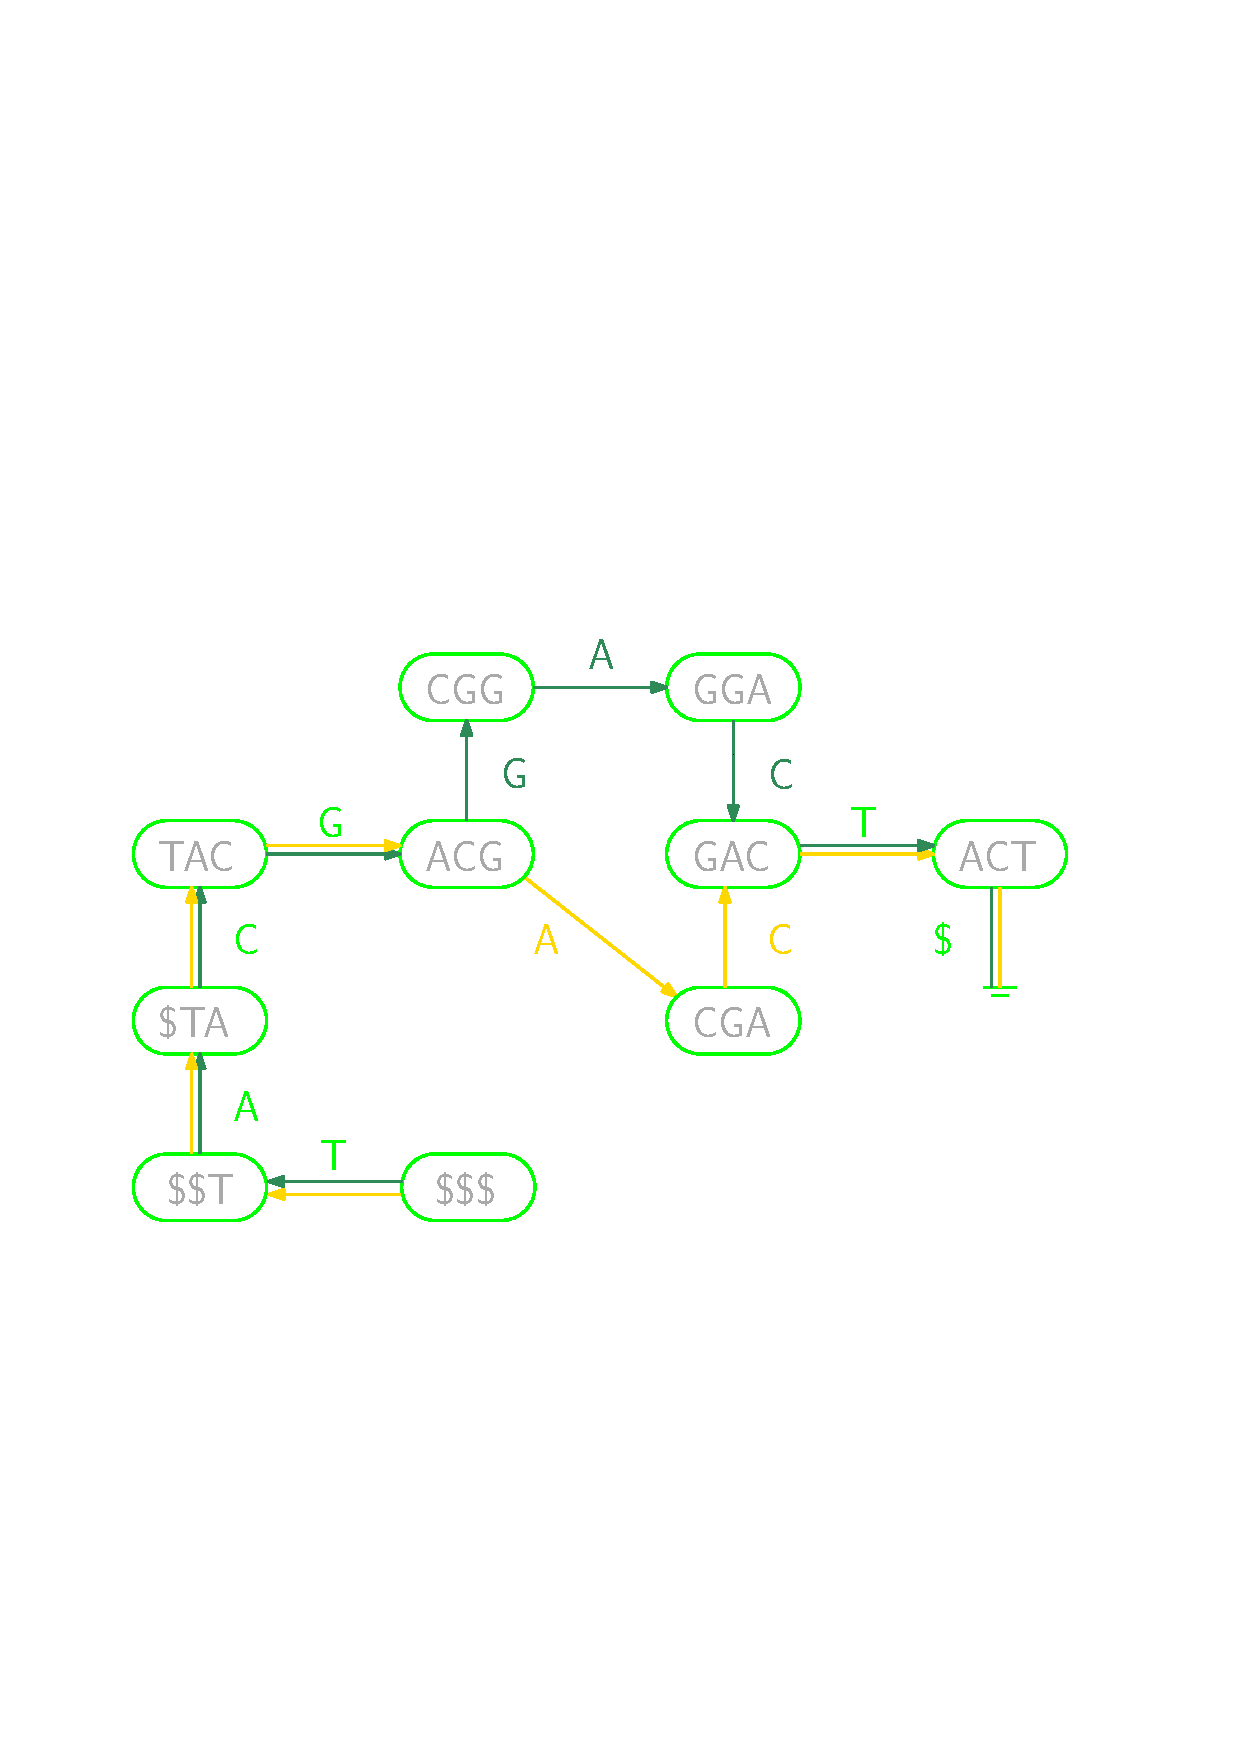
\includegraphics[width=.35\textwidth]{limegraph.pdf} \\~\\
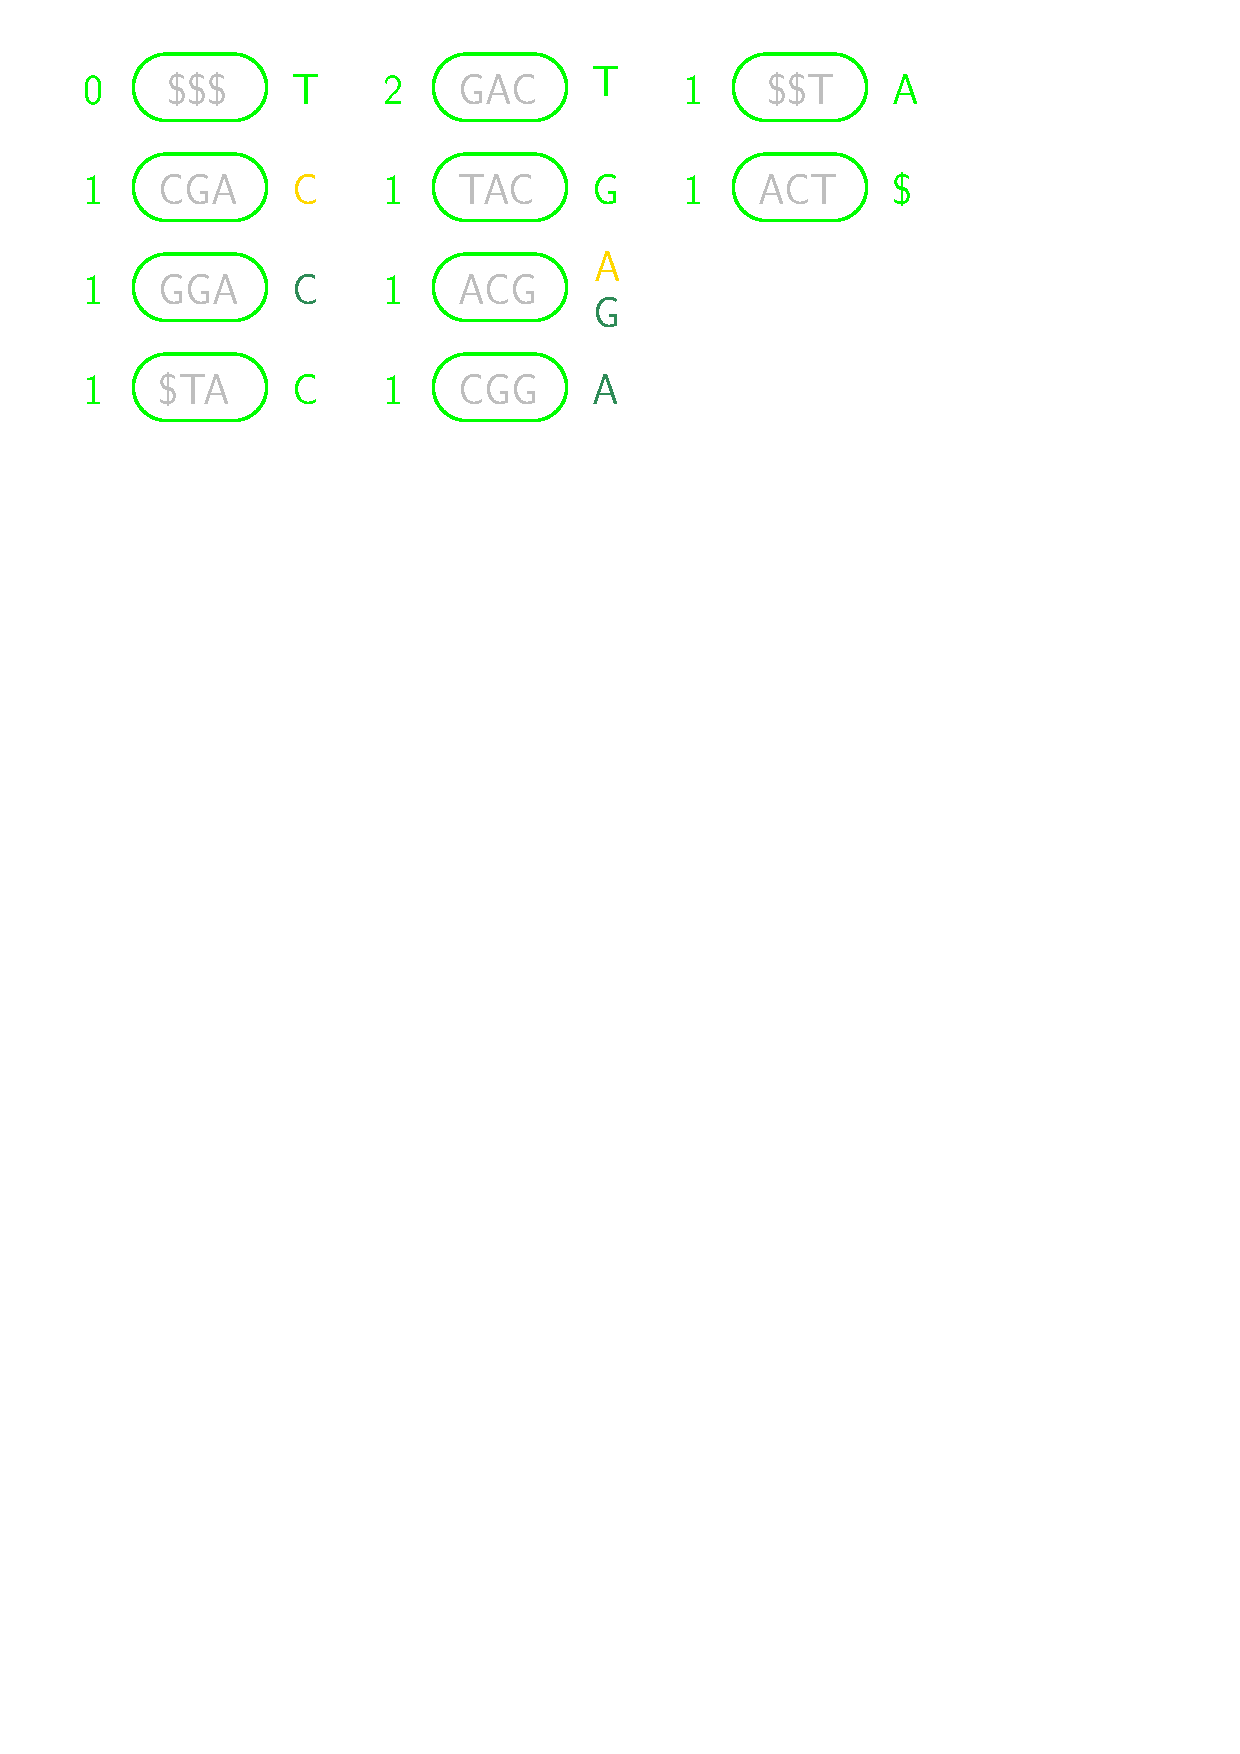
\includegraphics[width=.35\textwidth]{limeonlymapping.pdf} \\~\\
\raisebox{0.1ex}{$\begin{array}{rr}
   \EBWT (G) = &  \mathtt{TCCCTGAGAA\$}\\[1ex]
         \B_F = & \mathtt{ 1110111111}\\
         \B_L = & \mathtt{11111101111}\\[1ex]
C^\mathrm{T} = &   \mathtt{11011110011}\\
               &  \mathtt{10111101111}
\end{array}$}
%\end{tabular}
\caption{{\bf Top:} A colored de Bruijn graph consisting of two individual graphs, whose edges are shown in yellow and green. All nodes to be present in both graphs are shown in lime.  {\bf Below:} The $\vari$ representation of the colored de Bruijn graph: the edge-BWT and bitvectors for the union of the individual graphs, and the binary array $C$ (shown transposed) whose bits indicate which edges are present in which individual graphs.}
\label{fig:purple}
\end{figure}


\section{Do Novo Assembly}

In this section, we'll review tools that are capable of \emph{de novo} assembly, which means they attempt to reconstruct the genome using only a set of reads, as opposed to reference based tools which we'll discuss later.

\subsection{Overlap Layout Consensus}

\subsubsection{DALIGN}

DALIGN offers a solution for efficiently aligning pairs of PacBio RS II reads, which can subsequently be used in an overlap-layout-consensus assembler \cite{myers2014efficient}.
These reads are much longer than Illumina reads averaging 10 Kbp in length, but have a relatively high error rate at approximately 15\%  \cite{quail2012tale,myers2014efficient}.  
This is important, as de Bruijn graph based assemblers would not work with such a high error rate.
%** filter (seed)

DALIGN follows a ``seed and extend'' approach where exact substring matches known as seeds are found and then an error tolerant process is used to extend the matches.
Reads are divided into 14-mers.
They show that for PacBio data, over 99\% of high quality alignments between read pairs will have at least three 14-mers conserved.
They use this principle to build a filter, reducing the number of read pairs that must be aligned through their subsequent, more specific but computationally expensive, approach.
They additionally improve the specificity of this filter by limiting candidates to those where the conserved $k$-mers would all exist within the same diagonal band in a dynamic programming matrix and threshold matches on the number of bases in conserved $k$-mers. %fixme: do they always use 14-mers? if so, say that
This latter threshold is to address the issue that three consecutive conserved $k$-mers would share a run of k+2 bases which is not as specific as three non-overlapping conserved $k$-mers.
%These shared $k$-mers become seeds which are then used in a bounded, iterative deepening, depth first search to extend these matches.

DALIGN sorts these 14-mers to find seed matches using the author's own sort algorithm, carefully tuned for modern caching multicore processors, to find read pairs with shared $k$-mers.
%** sorting
%fixme
%** extending

DALIGN then extends matching seeds by incrementally extending promising paths from the ends of the seeds in a bounded, iterative deepening, depth first search.
The author describes this process as follows: first, they define the furthest reaching points, which are points on diagonals with the farthest anti-diagonal that have some exact cost (given an assignment of penalties for the different edit operations), \emph{d}.
They show how the furthest reaching point with  $d+1$ errors can be found using the furthest reaching point with $d$ errors.
Each set of $d$ furthest reaching points forms a wavefront, and computing successive wavefronts comprising furthest reaching points with additional errors can be seen as a wave, moving diagonally through a dynamic programming matrix.
This wave is pruned using two principles: a.) Any good alignment path will, in a dynamic programming matrix,  not have an excessive error rate over any reasonably large series of columns (the ``regional alignment quality criterion"), and b.) wavefront points that lag too far behind the leading point are also not likely to be on the optimal path.
Paths are extended until they either reach the boundary of the D.P. matrix, or all the points would be trimmed by \emph{a}.
In the latter case, the path is shortened to a \emph{polished point} as the criterion for allowing a path to continue growing is overly permissive.
These polished points satisfy the criterion that every suffix of the path satisfies a certain alignment quality threshold.  %(fixme polish algorithm)

Because the PacBio reads are much longer than those from the more pervasive Illumina sequencing platform, they can span longer repeats leading to more complete assembly.
%commentary

\paragraph{Discussion}

One area of potential further exploration is how sequencing depth affects the assembly problem.  There is likely a tradeoff between availability of read data and necessary alignment quality cutoffs.  With higher coverage, higher quality alignments could be required by the algorithm, which would allow more aggressive pruning of the search space during extension.  Conversely, more reads would introduce more seed matches and thus more extension operations to perform even if they can be computed faster.  

One way this approach might be improved upon for the purpose of assembly is to more closely couple the alignment to the assembly.  Given that 85\% of the time is spent extending alignments, speed improvements can either come from a more specific filter, or faster extension itself if all alignments are to be found.  However, perhaps not all alignments need to be found.  In our consideration of the SGA assembler (to follow), transitive edges are removed from its string graph because they don't provide any additional information.  If two reads align, and the seeds indicate a third read might align to the already covered region of the prior two, then the third read would be discarded from the graph even if the alignment posited by the seeds holds after extension.  In this way, some of the alignment work can be pruned.

Additionally, keeping the focus on doing enough work for the end goal of assembly, some alignments may be extended longer than necessary.  One potential risk from pruning the alignment effort to what is absolutely required for a structurally correct assembly is that it will leave fewer aligned reads at each locus in the genome with which to form a consensus base call.  However, a structurally correct assembly with many small indels and substitutions could be refined.  It might be profitable to do so with another sequencing platform such as Illumina.  While the high error rate of the PacBio would be present in the assembly (albeit potentially lower in any cases with sufficient reads overlapping to have some consensus), the difference rate should be less than 16\% for aligning Illumina reads (with a 1\% error rate \cite{quail2012tale}) as opposed to the 30\% pairwise difference rate between PacBio reads.  Beyond the lower difference rate, an Illumina read set probably wouldn't need the same depth of coverage as is used for \emph{de novo} assembly and only needs to be aligned against the assembly which will be an order of magnitude smaller than a read set.  Also, if the correct structure can be assembled from a subset of read alignments, PacBio reads could still be used to refine it.  Again, such a strategy would benefit from the partial consensus having a lower error rate and the smaller target.  The lower error rate of the partial consensus itself might open the door to faster alignments of the remaining reads.

One could imagine an extreme example of building a graph based on seed matches alone and then using a continuum of progressively more specific but more expensive alignment refinements driven by the graph connectivity and simplification.  Though in this scenario, it means the read pairs undergoing the most expensive alignments would have already undergone all of the cheaper alignments, so the reduction it times doing the expensive alignments would need to offset the cost of all the cheaper alignments done when the full alignment was needed in the end.

\subsubsection{SGA}

SGA is an assembler that uses an FM-index to find overlaps between reads instead of the earlier all-pairs dynamic programming based alignment approach  \cite{simpson2010efficient}.  


The first stage consists of error correction.  The paper describes a $k$-mer frequency method, which uses an FM-index built on the reads for error correction which allows any $k$ value.% (fixme define this).
The FM-index is built by merging many smaller FM-indexs, one for each of many blocks of reads.
For whatever value is chosen, each $k$-mer within a read is checked to ensure there are enough other copies of the $k$-mer in the read set to support that it could be a genomic $k$-mer and not the result of a sequencing error.
If there is insufficient support, but a base within the $k$-mer can be replaced with a single other choice to produce a new $k$-mer with such support, the replacement is done.
Otherwise, error correction stops on this read.
%The other error corrector is based on overlaps with other reads (fixme: elaborate?).

After read errors are corrected, a new FM-index is built on the corrected reads.
In addition to correction,  duplicatate reads are removed and certain other reads are filtered out at this stage.%fixme: which
This can occur without rebuilding a third FM-index with a technique that allows  marking certain entries absent.

It then proceeds to find overlaps between reads with the new FM-index.
%(FIXME: talk about FM-index tricks, like hiding entries and merging FM-indexes). 
%fixme-clean: It exploits additional features of the FM-Index such as the ability to operate on compressed form of the text where runs of repeated symbols induced by the BWT are represented succinctly and the ability to merge two FM-indexes.  
The FM-index allows it to find exact matches in time linear to the number of reads (treating read length as bounded by a constant).

Next, it builds an overlap graph and simplifies it.
Overlapping reads can exist in a transitive relationship with each other, such that two reads that overlap each other both overlap some third read that covers the already overlapped region of the first two.
In such cases, the third read is clearly redundant to the completely covering sequence already conveyed in the first two.
Eliminating such redundant reads, %(FIXME-true? as well as any duplicate reads) 
results in a simplified overlap graph known as a \emph{string graph}.
SGA also provisions for multiple paths in the string graph that are consequence of heterozygosity (multiple different variants of the same gene, on different copies of a chromosome) and prunes down to one to further simplify the graph.
It then attempts to find Hamiltonian paths through this simplified graph which are emitted as contigs.

Finally, after contigs are formed, reads are aligned to the contigs and scaffolds are formed.
This is based on modern sequencing platforms which provide paired end reads.
Paired end reads are created by sequencing both ends of a larger fragment with an unsequenced DNA region in the middle of a known length.
If the left read of a read pair aligns to one contig and the right read aligns to another contig, the two contigs can be joined together into a \emph{scaffold} with a run of `N's in between denoting the length of DNA known to be present but of unknown sequence.
%Their results show that SGA uses less memory, takes more time, and generally produces better results than competing de Bruijn graph based assemblers.
They indicate that the largest time consumer is the construction of the FM-index itself, though this must only be done once for a read set and allows multiple experimental runs to optimize the parameters.% (min-overlap, + FIXME what else). 

% commentary
\paragraph{Discussion}

The SGA authors advocate that their approach allows parameters such as the min-overlap (which paralles to $k$-mer size in a de Bruijn graph approach) to be optimized cheaply.  Methods we will discuss later, such as the variable order de Bruijn graph (and assembly algorithms that can use it) as well as predictive methods such as $k$-mer geanie may obviate the advantage for cheap parameter tuning.

This approach uses paired ends after initial assembly for scaffolding.  Given that overlap-layout-consensus assembly allows high error rate reads, an interesting question for further exploration would be if the entire fragments input to a sequencing platform be treated as reads (``fragment-reads'') with the unsequenced middle portion (runs of N's, flanked by left and right ``end-reads'' reads) be treated as a run of a combination of low penalty mismatch and insertion/deletion errors?  Thus the minimum overlap could span the unsequenced gap. Such alignments could be found either by the union of those left end-reads that have concordant right end-read alignments (each of left and right alignments found independently), or a special \emph{shortest-possible-insert} symbol added for index based alignment to reduce the time matching the long run of N's.

Although this assembler uses more CPU time than de Bruijn graph based assemblers, much of it is parallelizable (much like $k$-mer counting and sorting).  The read error correction phase is a perfect fit for the map-reduce computation infrastructure enjoying widespread cloud support.


%Critique: Can an OLC type assembler work in terms of whole fragments with variable length runs of N's in the middle (the insert)?

\subsection{de Bruijn Graph Assembly} %fixme: move to de novo section

%\section{Making the most of read data}
In this section, we'll look at several methods for de Bruijn graph based assemblers.  They contribute to making the most of whatever structure is discernable from a given read length, sometimes focusing on reducing assembly running time over other alternatives giving equivalent results.  

\subsubsection{Paired de Bruijn Graphs}

The paired de Bruijn graph \cite{medvedev2011paired} works to reduce the tangledness of a graph.
Tangles result when $k$-mers do not fully span repeated regions and thus $k$-mers from reads from disparate loci in the genome are glued together.

They mention that some of these tangles can be resolved during traversal by limiting it to paths that agree with the mate pair, but this has problems.
One way the tangles can be prevented is to keep track of the reads form which $k$-mers originated, and check that there is some evidence of overlap in the mate pairs before gluing.
This is true because if both left reads were read from the same locus in the genome, then their right reads (with differences due to variances in exact insert size between a read pair) would also be read from a common locus.
They check for this property by searching for a short path between $k$-mers drawn from the same  relative position in the right reads within a de Bruijn graph.  
%todocommentary:paired

\paragraph{Discussion}

Using $k$-mers from the right reads to decide gluing of $k$-mers from the left read is a relatively cheap heuristic to determine whether the potentially glued $k$-mers are read from the same locus.  This ignores all the other bases in the read and whether they support or contradict the notion the left $k$-mers were sequenced from the same locus.  A more specific alignment criteria may detangle graphs even more.  Even if more computationally expensive, it could be applied to only those $k$-mers involved in tangled regions of the graph.
%Commentary: Are there fast, more robust estimates to whether the left pair have concordant right pair?  What about the other bases in the read? Presumably this method is cheaper/smaller.

\subsubsection{$k$-mer Genie}

$k$-mer genie is a tool for predicting the $k$-mer size parameter leading to optimal assembly from a de Bruijn graph based assembler \cite{chikhi2013informed}.

It notes that too small of a $k$-mer leads to an overly tangled graph, while too large of a $k$-mer leads to a disconnected graph.
While trying all possible $k$-mer sizes is possible, a single assembly with a given $k$-mer value can take several days, so exhaustive search may be prohibitively expensive in terms of time.
They describe two main ideas useful for selecting an optimal $k$-mer size: A $k$-mer abundance histogram (explained momentarily) which an expert may use, and the heuristic that the $k$-mer size resulting in the most diverse set of genomic $k$-mers present in reads will lead to optimal assembly.
A $k$-mer abundance histogram can be generated from $k$-mer counts and indicates for each $k$-mer frequency, how many distinct $k$-mers had that frequency.
As $k$-mer counting itself is computationally expensive, they give a method for sampling a fraction of all $k$-mers and inferring an abundance histogram from the samples.
This is asymptotically the same as a full $k$-mer abundance histogram but results in lower constant factors, making it useful in practice.
They then describe the application of a generative statistical model, whose parameters can be tuned to match the measured abundance histogram.
These parameters then provide a maximum likelihood  estimate for which $k$-mers in the abundance histogram are genomic $k$-mers vs. the result of sequencing errors.
The $k$-mer size with the most distinct genomic $k$-mers is believed to lead to the best assembly, because too large of $k$-mers (near the read length) will likely miss some genomic $k$-mers due to incomplete coverage, while too small of a $k$-mer size will lead to different regions of the genome having the same kmer (i.e. $k$-mers smaller than repeats of a given size will represent all occurrences of the repeat as the same $k$-mer).

\paragraph{Discussion}

As mentioned in our section on variable order de Bruijn graphs, some modern assemblers use multiple k-values.  The work here might might be extended to provide a set of promising \emph{k} values for such assemblers.  Though SGA authors argue their approach makes the search for optimal minimum overlap parameter cheap, it may be interesting if this approach can eliminate that search.
%todocommentary:$k$-mer genie
%commentary: note SGA's fast min-overlap size change. Interesting if efficient $k$-mer counters can become competitive with sampling used in $k$-mer genie.  Also, if LCP type operation with fm-index can substitue hash type kmer counts.



\section{Reference based assembly}

In this section, we review tools which use some kind of whole-genome reference to aid in reconstruction of a genome.  This can be a single reference genome for a species, a collection of multiply aligned genomes, or a maturing technology known as optical mapping. 

Optical mapping works by elongating large DNA molecules on a microscope slide and then cleaving them using restriction enzymes where ever the enzyme's recognition sequence occurs within the DNA molecules \cite{ORMenc}.
The breaks are visible under a microscope, and the DNA span between them can be estimated, giving a map of where the recognition sequence occured within the molecule.
Though this building a genome map with this system itself involves an assembly process, because of the much longer ``read'' length of the individual molecules (250-800 Kbp), near-complete automated assembly is often possible such that a map of all restriction sites across an entire genome can be produced.  Optical mapping has the potential to resolve many of the repeat resolution problems that occur with even the longest read lengths on the horizon.

\subsection{Reassembly}

A common task for biologists studying an individual's genome is resequencing, which uses a reference genome from a different individual in the same species.
Reference genomes can contain structure not found in a \emph{de novo}, as contigs are refined and relationships between them are resolved through a laboratory process known as finishing.
Resequencing works by aligning reads directly to the reference genome, under the assumption that the structure of the donor individual is the same as that of the reference.
This biases the results toward the reference and cannot necessarily detect or resolve structural variations even if a \emph{de novo} assembly of the donor reads could reveal one.
%fixme: move the above paragraph out of this section

In contrast, the work of Parrish, et al. \cite{parrish2013genome} uses the already resolved structure in a reference genome, but only to guide the traversal of otherwise ambiguous choices in the traversal of a de Bruijn graph built from donor reads.
The idea is that the structure of an individual's genome (referred to as the donor) will be similar to a well-chosen reference genome, and thus the donor genome's structure can be inferred using the most parsimonious traversal of the graph with the reference genome in mind.

They argue that finding the truly most parsimonious traversal is hard, so they solve the easier problem of finding traversals spelling out sequences that deviate from the reference by at most $\tau$ consecutive bases.
Finding such traversals proceeds as follows: First, they glue nodes between the donor's de Bruijn graph and that of the reference but preserve the edges.
Then, they define parallel edges in this graph for each donor $k$-mer edge that is also found in the reference genome.
The presence of a reference edge parallel to a donor edge is actually represented as a donor edge annotated with the reference edge's $k$-mer position in the reference genome.  

This initial graph is modified to make traversal easier.
Nonbranching paths with a consistent (i.e. reference positions incrementing/decrementing one position per edge) sequence of parallel edge positions are condensed into a single edge which is then annotated with the corresponding interval in the reference genome instead of a single position.  

To aid traversal satisfying the $\tau$ limit, they add reachability annotations to non-parallel edges.% (fixme: lookup their name for these).
Specifically, they infer what the reference position would be for adjacent edges, annotating the inferred position on them.
This process is then repeated to propagate inferred positions onto successively further adjacent edges.
These inferred, non-parallel, positions represent deviations from the reference which must not exceed $\tau$, so each propagation keeps track of how many non-parallel edges the inferred information has traveled past.
The propagation terminates when this exceeds $\tau$.
Inferred position markers are then pruned if consecutive markers are not connected (concordant).

%commentary: 

\paragraph{Discussion}

The novelty of this approach can be expressed in terms of what relationships are used.  \emph{do novo} assembly is based exclusively on the relationship of reads to each other. Resequencing is based only on the relationship of reads to a reference genome.  This approach uses both.  This approach has clear parallels to AGORA, which uses optical maps in place of a reference gnome.   AGORA has an advantage in that it would likely be used with an optical map (which reveals to the limits of its resolution the structure) for the donor genome,  so there would be no risk of bias toward a different structure that might occur in the reference genome.  This reassembly method has an advantage in that the reference genome captures the structure down to the nucleotide level resolution, where as optical maps minimum resolution is about 1 Kbp.  This work could be extended to include both the donor's optical map and the refernce genome.

The quality of the resulting structure could potentially be enhanced by bayesian inference.  A collection of known structural variations for a population (discussed again in our section on GCSA) and their frequency could be used as our prior belief about the structure of a donor's genome, then a posterior probability of a given structural variation could be calculated based on the observed sequence reads and their assembly.

\subsection{GCSA}

The Generalized Compressed Suffix Array (GCSA) is a data structure that stores a compressed index of a finite state automata \cite{siren2014indexing}.
Among other uses, such automata can represent a collection of known structural variations across a population.
There is an advantage of having auxiliary data source be as similar as possible to the data of an individual's genome being assembled.  By representing a large sample of structural variations in a way that allows them to be independently combined, there is a greater chance some combination will match a particular individual.
Consider a simple directed graph representing a canonical individual from some population as a linear alternation of labeled vertices and edges connecting them.
This simple graph forms the basis for a more complicated one and the single original path through this initial graph, after the graph is expanded, is called the \emph{backbone}.
Then, any variation relative to this graph can be represented by adding additional paths: those that skip backbone nodes for deletions, those that add additional nodes for insertions, and those that provide an alternative subpath around backbone nodes for substitution.  

This graph can be treated as an automaton for path matching, where a string of symbols spells a path of node labels.
The initial automaton is reverse determinized and prefix sorted such that it can form an automaton represented by a compressed suffix array (FM-index) and auxiliary bit vectors encoding the forking and joining of paths.  This structure allow paths to be matched in reverse without backtracking.

To help understand how an FM-index can represent a graph, consider a FM-index of a string as a special case under this generalization.
It is equivalent to the backbone path alone.
Since any node in such a graph can only be followed by the one path to the terminal node, such nodes represent complete suffixes.
The FM-Index procedure \emph{backward search} finds successive, possibly smaller intervals in a BWT which exactly match successively longer suffixes of a query string. It allows stepping backward through this graph one edge at a time (though actually doing all matching suffixes in parallel, so following multiple edges, one for each match `in flight'). %fixme: move to FM-index section, part of it
For a traditional FM-index, backward search maintains the invariant that all suffixes in the interval exactly and completely match the suffix of the query matched so far.
In contrast, in GCSA, there may be multiple paths forward from a given node, so a node represents only the shared prefix which is guaranteed among all paths forward from that node.
Thus, for an FM-index backward search  the invariant is that the set of nodes in the backward search interval are each consistent with the portion of the query string matched up to that point.  

Some of these nodes may denote prefixes longer than the matched suffix of the query, or the matched query suffix may be longer than the definite prefix denoted by a node.
It might help to think of a query as having an infinite string of N's following it and each node as well having an infinite string of N's following its label (n.b. not all nodes that would match will necessarily be in an interval late in the search, as previously matched query symbols may restrict the nodes in the interval to just those with outgoing edges that would lead to the longer suffix than just the portion definitely matched by that node.) 

Up till this point, we've only considered exact matching, but just as with traditional FM-index backward search, this can be extended with backtracking search to allow insertions, deletions, and substitutions so inexact path matches can be found.
Their implementation provides this option, using the BWA algorithm.% \cite{durbin}
%commentary

\paragraph{Discussion}

This approach helps resolve some of the problem of bias toward a single reference genome mentioned for reassembly and resequencing, as with a sufficiently large population, most of the variations present in the whole population may have already been resolved.  It does leave two important issues: First, the true structure of each individual in the reference set has to be determined correctly, and second it needs to be multiply aligned somehow.  

It would be interesting if this could be used online, such that a new individual aligned against the set but with new structural variations would modify the reference set to include the new paths.  

Again, this task would require good enough \emph{do novo} information to reveal a novel structural variation in the first place.  Given the smaller read set in resequencing, the less abundant information might not be enough to unambiguously resolve the structure of all possibilities in the read set, but still be enough to constrain to one possible variation from the set of all known SVs.  

GCSA may have some limitations: Supposing half of a population has a particular translocation, but one individual has novel a duplication; GCSA has no constraints to identify this and would match the new individual despite the presence of a potentially important structural variation. This is of course a limitation of the finite languages an automaton can represent, and might be addressed with a context free grammar of genomic structures.  This work could be extended by capturing the observed combinations of structural variations, possibly in a machine learning model given that we don't know exactly what the rules are, such that particularly deviant ones (such as in a disease population) might be flagged as anomalous.  This has parallels in the natural language world where grammatical sentence structure can be learned and subsequently used for identifying ungrammatical sentences.

%Resequencing problem of no-place-to-put-novel-structure should be moot if all SVs are captured in the population.  

\subsection{SOMA}

SOMA is a tool developed  by Nagarajan \emph{et al.} \cite{nagarajan2008}. They focus on the problem of scaffolding and validating contigs for bacterial genomes.
Both of these tasks require first finding alignments between contigs and an optical map.
These alignments can be found by \emph{in silico} digesting contigs, that is, locating the restriction enzyme's recognition sequence within the contigs and counting bases between occurrences, where these counts become the \emph{in silico} fragment sizes.
Then alignments can be found using dynamic programming, using an appropriate error model and recurrance function. 

They model the error in estimating the enzyme cleaved fragments' sizes as a normal distribution and use a $\chi^2$ scoring function for one component of the alignment score between two sequences of fragment sizes.
They discuss the possibility that sequencing errors could cause missing cut sites in the \emph{in silico} digested contigs, but their preliminary experiments indicate that considering all occurrences of near matches with the enzyme’s recognition sequence produces too many false positives.
Instead, they include this possibility in their scoring function.

Their scoring function has two primary components: Alignments with more matching restriction sites are considered better, and between alignments with the same number of matching restriction sites, a smaller χ score is better.

Their dynamic programming algorithm is formulated from three components, the previous best matching cut site score, a function of the putative false or missing cuts between the previous best score cell and the current cell, and the degree of agreement between the sizes of the region that spans these two cells.
The number of false or missing cut sites is penalized by a constant factor.
The degree of agreement is the difference in the sums of the fragment sizes for each region divided by the sum of the squared standard deviations of the optical map.
Unlike other approaches, they do not limit the search for the previous match site to just a small number of missed cut sites, but search back to the beginning of the dynamic programming table.
This means the algorithm has complexity O($m^2n^2$).
They suggest that this search could be pruned using the fact that they expect the sum of the sizes of fragments to agree well.

They mentioned that there are several other considerations for the alignment problem which they addressed in their software.
First, fragments smaller than 700 bases are typically not captured in the optical mapping process.
Second, the ends of fragment sequences are usually not the result of restriction enzyme digestion.
Finally, bacterial chromosomes can have a circular map, so care must be taken to allow alignments that span the ends of a linearized map.
Their dynamic programming algorithm will find an optimal alignment score for any contig, even those that do not belong to the genome.
They suggest that a threshold value could be used to discriminate between alignments considered valid or otherwise, but that this value would likely depend on the length of the sequences being matched.
They propose comparing the match score to the match scores of random permutations of the \emph{in silico} digested contig’s fragments.
Then they can use a P-value from this permutation test (the probability that a random match has a higher score) instead of a constant threshold.
As they are concerned with scaffolding and placement, they also filter the possible alignments for contigs to those that are among the best of those that are good enough to be considered possible.
They then cast the assignment of loci to the contigs as an operations research problem called interval scheduling.
In this way, they are able to find placements for all correctly assembled contigs such that contigs are placed in one of the alignments where they score well, and no two contigs are placed in an overlapping fashion.
This problem is NP-complete, so they use a greedy heuristic and demonstrate that on small genomes this works well in practice.
%They test their algorithm on both simulated data where the correct results are known as well as on real data.


%commentary

\paragraph{Discussion}

SOMA's biggest limitation is that it runs after assembly has already taken place, so while it can detect some misassembled contigs, had the same structural information contained in the optical map been available during assembly, it could have guided the assembler on the correct path in the assembly graph.  Also, because of the complexity of its dynamic programming algorithm it only practical for prokaryote scale genomes.

%% Relevance: The SOMA tool includes alignment of contigs
%% to an optical map, so they are in fact solving the same problem we
%% are.

%% Remaining work: While the authors have demonstrated
%% the effectiveness of SOMA on prokaryotes, their algorithm has
%% runtime complexity aproximately proportional to O(m4) and so like
%% the previous work will not scale to eukaryote sized genomes.

\subsection{AGORA}

Another tool, AGORA by Lin et al. \cite{lin2012agora}, uses alignment of sequence data to optical maps to guide assembly.
It works on the premise that when an assembler is traversing a de Bruijn graph in an order that “spells” the genome sequence, then an \emph{in silico} digest of the bases along that path should also align to some part of optical map.
If a potential path through the de Bruijn graph cannot be aligned anywhere on an optical map, then it can be discarded as not genomic.
In this way, the graph traversal is restricted to only those paths that agree with the information provided by the optical map.
In principle, this leads to computationally intractable problems, but the authors demonstrate that heuristics can solve the problem effectively for bacterial genomes.

One of the essential ideas in their traversal is the concept of a landmark.
These are edges in the de Bruijn graph that uniquely align within the optical map.
The search for paths through the de Bruijn graph begin with these landmarks.
Then an attempt is made to find a path through the graph between landmarks that matches the span between them in the optical map.
Specifically, they perform a depth first search from each landmark, checking at each step if the path thus far is consistent with the optical map.
They note that while this can lead to multiple paths, generally the paths are similar except for small complex repeat regions.

%% To test their algorithm, they used reference genomes from 369 bacterial genomes and generated simulated optical maps with three levels of error (high, medium, low).
%% The high level was characterized based on data from a real optical map of Y. pestis KIM.
%% They also generated error-free de Bruijn graphs from the reference genomes.
%% Using AGORA, they were able to achieve 98\% sequence correctness on 3/4 of the genomes on all three error levels.
%% They additionally tried using a real optical map of Y. pestis KIM on a simulated de Bruijn graph, and found that the assembly quality was slightly worse than when using their high error level simulated map, suggesting their error simulation may not have captured all of the important characteristics of real data.

They implemented a simple greedy algorithm to align sequence data to optical maps because existing algorithms have prohibitive runtime complexity.
Their alignment algorithm compares fragments between the two sequences in order and does not allow for restriction site errors (presence or absence) in the optical map.
It does allow for different fragment sizes to account for sizing errors, and removes all fragments that are small enough to sometimes be missed completely in the optical map.
When no landmark edges are found, they look for pairs of consecutive edges in the de Bruijn graph that have a unique alignment in the optical map.

%% They also analyze the affect of enzyme choice.
%% They found enzymes that cut frequently, combined with low error rate allowed AGORA to produce the best assemblies.
%% This did not hold for higher error rates, and the authors conclude the is due to small fragment loss.

%commentary

\paragraph{Discussion}

Though their work is promising, there are a few areas for caution.  They acknowledge that their heuristics may not be effective on real data. Since they use a greedy algorithm to match \emph{in silico} digested sequence data to an optical map, the real-world sources of error would cause their matching algorithm to miss correct alignments. Additionally, as with SOMA, optical maps have limited resolution (typically no finer than 1 Kbp) and the inherent optical map fragment sizing error means many spurious paths may also align, particularly with larger genomes which will more densely populate the possible fragment size patterns.

%Also, while some portions of contigs will certainly align to an optical map, this only holds for those containing sequences that align to only one locus in an optical map. This means their contigs may still have regions where their construction was not guided by the optical map and may disagree, hence indicating a possible misassembly.
%todocommentary:agora
%Relevance: The AGORA tool includes alignment of sequence data to optical maps. They attempt to produces assemblies where contigs are generated in such a way that they match an optical map. One would expect such contigs to always align to an optical map since they were generated this way. In this way, they are also concerned with misassembly and potentially produce fewer misassembled contigs when the optical map is able to guide the de Bruijn graph traversal so as not to produce them. Additionally, we explore matches accounting only for sizing errors, so this is another similarity to our work.

%Remaining work: They acknowledge that their herustics may not be effective on real data. Since they use a greedy algorithm to match \emph{in silico} digested sequence data to an optical map, the real-world sources of error would cause their matching algorithm to miss correct alignments. Also, while some portions of contigs will certainly align to an optical map, this only holds for those containing sequences that align to only one loci in an optical map. This means their contigs may still have regions where their construction was not guided by the optical map and may disagree, hence indicating a possible misassembly.


\section{Memory/Time Efficient Data Structures}

In this section, we review modern data structures which facilitate accomplishing tasks already shown to produce valuable results but with fewer resources used.  This class of research is valuable because it allows state of the art existing solutions to be employed by biologists with modest only computing resources, as well as extending the reach to ever larger genomes and tasks for large labs with vast computing resources.

\subsection{KMC 2}

Deorowicz \emph{et al.} \cite{deorowicz2015kmc} introduce a new tool which extends previous work with minimizers (explained shortly).
This paper addresses the problem of how to efficiently count $k$-mers in a read set.
$k$-mer counting is important as only high frequency $k$-mers are likely to be genomic, and those that drastically exceed sequencing depth can be used as weights in a de Bruijn graph and indicate genomic repeats.  The extent of the deviation, for example, can convey copy number for tandem repeats.

This work improves upon the memory and CPU consumption of an earlier work which is also a minimizer based $k$-mer counter.
A minimizer is the lowest ranking m-mers ($m < k$) of all m-mers within a $k$-mer, according to some ranking system (e.g. lexicographic).  Many consecutive $k$-mers share the same minimizer, and it can be expected that all occurrences of any of those $k$-mers across the whole read set will have the same m-mer.
Thus, by distributing these consecutive $k$-mers (or more efficiently, the covering span of bases across all such $k$-mers with the same minimizer as one contiguous unit called a \emph{super $k$-mer}) into different bins, identical k-mers can be grouped.  In this scenario each bin is associated with a subset of all minimizers, all $k$-mers across the read set will be stored in the same bin as all of other copies of identical $k$-mers.
Each bin can be processed independently using a subset of the memory required for for the complete set, and the union of all counts constructed at the end.

This method improves on the aforementioned process in two ways:

First, the peak memory will occur with the largest bin, and a lexicographic ordering does not yield a uniform distribution, so they provide a new ranking scheme such that certain problematic m-mers, particularly prefixes of consecutive 'A's do not skew the distribution (a problem observed by several researchers).
They dub m-mers chosen under this scheme \emph{signatures}, which are still minimizers under the original definition, but which favor some specific desirable properties such as producing more uniform bins and reducing disk I/O.


Second, after being split into bins and a given bin loaded from disk, super $k$-mers are not entirely split into $k$-mers as with previous approaches, but instead into varying length substrings known as (k,x)-mers.
These vary in size $k$..$k+x$ which eliminate some of the redundancy of extracting all $k$-mers, since the longer strings contain multiple overlapping $k$-mers.
These ($k,x$)-mers are then sorted, and multiple cursors iterate through to count the $k$-mers.
Note that the $k$ sized suffixes of the sorted ($k,x$)-mers which share the same prefix will be stored consecutively, but will be found in $\sigma^{[0..x]}$ different places in the sorted sequence in addition to the one run where they exist as a prefixes.
%todocomentary:kmc 2

%Commentary: 

\paragraph{Discussion}

There is some similarity between the kmer counting work done here for minimizers and that done by DALIGN's sorting and SGA's index building; In each case, the large set is divided into (possibly similar, \emph{independent} smaller chunks which are processed either one at a time (due to memory constraints) or concurrently (where independence entails the useful property of being synchronization free) and are later merged.

\subsection{Variable Order de Bruijn Graphs}

Two state-of-the-art assemblers, SPAdes and IDBA, consume significant time building de Bruijn graphs of different orders as part of their operation.
The work of \cite{boucher2014variable} attempts to address this burdon.
This approach introduces a data structure which is both succinct and can represent all orders of de Bruijn graphs up to some maximum size in a single structure.
It is an extension of a previous succinct de Bruijn graph representation called BOSS (for the authors' initials) and works as follows: Given a set of 2-tuples, each of the $k-1$ symbol prefix and the 1 symbol suffix of each $k$-mer (representing a vertex and an outgoing edge, respectively) the structure stores a fixed order de Bruijn graph as a sequence of these tuples, sorted first in right to left order of the prefix and then by suffix.
As each node may have up to $\sigma$ outgoing edges, nodes are represented by an interval of all such tuples.
Three operations are provided: forward (taking a node and an edge symbol to follow and returning a node), backward (returning all preceding nodes of a given node), and lastchar (taking a node and returning a symbol).
A node's complete label can be determined by successive calls to backward and lastchar.  

The authors then discuss extensions to this representation, supporting smaller values of $k$.
They point out that if the first column of the prefixes were removed, the data structure would be quite similar to the BOSS of order but one degree smaller (though it would have some repeated rows).
The original operations will not work correctly all the time on this reduced order \emph{view} of the BOSS so additional operations are provided: shorter, longer, and maxlen.
The functionality of the original operations can be expressed in terms of this new set, by mapping a smaller order node to an equivalent maximum order node, calling the original operation, then mapping the result(s) back to the appropriate small order node.
%commentary

\paragraph{Discussion}

Much like KMC 2, this approach reduces redundancy by leveraging the fact that a lexicographically sorted sequence of strings also has one or more sequences of sorted subsequences within it.  If left-to-right sorted, removing a suffix elementwise leaves a sequence in sorted order with possibly new repititions.  Removing a prefix of length $l$ leaves a series of $\sigma^l$ sorted sequences.  In KMC 2, both prefix and suffix strings are of interest so the disparate sorted sequences found by ignoring a prefix must be traversed while the variable order de Bruijn graph only removes the equivalent of suffixes (actually prefixes, being right-to-left sorted.)


%todocommentary:variable order
%Commentary: could the out edge suffix be interposed before the rightmost optional column and the leftmost permanent column?  Then truncating columns would still be in lex order.




\chapter{Conclusions}
\label{sec:conclusions}

%\section{Future Work}
%\label{sec:future-work}


\section{Acknowledgements}
The author would like to thank Mark Heim and Basir Shariat Razavi for editorial assistance provided in the form of annotating a draft of this document with grammatical and typesetting errors as well as highlighting areas that didn't make sense to them. The ideas expressed in the summaries are obviously those of the authors of the individual works.  The ideas in the background are long standing ones applied in the field of Bioinformatics and major ones cited.  The composition of all text was done by this author.

\bibliographystyle{splncs}

\bibliography{research_exam}

\end{document}
